\documentclass[12pt,a4paper,openright,twoside]{book}
\usepackage[utf8]{inputenc}
\usepackage{disi-thesis}
\usepackage{code-lstlistings}
\usepackage{notes}
\usepackage{shortcuts}
\usepackage{acronym}
\usepackage{listings-rust}
\usepackage{svg}
\usepackage{epstopdf}
\usepackage{cleveref}
\epstopdfDeclareGraphicsRule{.svg}{pdf}{.pdf}{%
    inkscape -z -D --file=#1 --export-pdf=\OutputFile
}
\AppendGraphicsExtensions{.svg}

\school{\unibo}
\programme{MSc in Computer Science and Engineering}
\title{Design and development of a Rust-based execution platform for Aggregate Computing}
\author{Micelli Leonardo}
\date{\today}
\subject{Pervasive Computing}
\supervisor{Prof. Viroli Mirko}
\cosupervisor{Dott. Aguzzi Gianluca}
\session{IV}
\academicyear{2022-2023}

% Definition of acronyms
\acrodef{iot}[IoT]{Internet of Things}
\acrodef{vm}[VM]{Virtual Machine}
\acrodef{ac}[AC]{Aggregate Computing}
\acrodef{fc}[FC]{Field Calculus}
\acrodef{cps}[CPS]{Cyber-Physical Systems}
\acrodef{cas}[CAS]{Collective Adaptive Systems}
\acrodef{jvm}[JVM]{Java Virtual Machine}
\acrodef{dsl}[DSL]{Domain Specific Language}
\acrodef{ast}[AST]{Abstract Syntax Tree}
\acrodef{pc}[PC]{Pervasive Computing}
\acrodef{rfid}[RFID]{Radio-Frequency Identification Technology}
\acrodef{fp}[FP]{Functional Programming}
\acrodef{scafi}[ScaFi]{Scala Fields}
\acrodef{rufi}[RuFi]{Rust Fields}


\mainlinespacing{1.241} % line spacing in main matter, comment to default (1)

\begin{document}

\frontmatter\frontispiece

\begin{abstract}
    The rapid expansion of the Internet of Things has led to the proliferation of computational resources in the physical world, which are now embedded in everyday objects and environments.
    The Aggregate Computing paradigm has emerged as a promising approach to tackle the complexity of designing and coordinating these systems, by shifting the focus from individual devices to
    programming the global behavior of whole computational collectives. The current state-of-the-art implementation of this paradigm is \ac{scafi}, which targets the Java Virtual Machine.
    Concurrently, the \ac{rufi} project aims to exploit the Rust programming language's features to provide a more lightweight and memory-efficient implementation of Aggregate Computing that can be executed inside resource-constrained, ``thin'' devices.
    In this paper, we will present the design and development of a Rust-based platform that will enable the distributed execution of \ac{rufi}-based aggregate programs, taking a step towards the goal of bringing aggregate computing to thin devices.
\end{abstract}

\begin{dedication} % this is optional
    ‘‘The most profound technologies are those that disappear. They
    weave themselves into the fabric of everyday life until they are
    indistinguishable from it.’’
    \begin{flushright}
        (Mark Weiser, 1991)
    \end{flushright}
\end{dedication}

\begin{acknowledgements} % this is optional
    I would like to express my deepest gratitude to my supervisor, Prof. Mirko Viroli, for his guidance and support throughout the development of this thesis.
    I also could not have undertaken this project without the support of my supervisor, Doct. Gianluca Aguzzi and the valuable advice and time he dedicated to me.
    I am also grateful to Doct. Nicolas Farabegoli and professors Roberto Casadei and Danilo Pianini for their help and support.
    A special thanks go to my group of friends first and colleagues later, the `Angels`'': Angelo, Paolo, Davide, Angela, Filippo, Eddie and Francesco.
    I would also like to thank my dear friend and fellow rustacean and gymbro Luca, as well as all the people who have been close to me during my years in Cesena: Massimo, Marco, Schiaro, Riccardo, Andrea and
    all the amazing people I met during this wonderful adventure.
    I'm also grateful to my amazing group of friends at home, my ``Branco'': Dona, Cristian, Riki, Claudio, Francesco, Simone, Aldo and Raffaele, we all met in childhood and have never been apart since.
    Last but not least, I would like to thank from the bottom of my heart my mother Simona and all of my family for being my best supporters and for always being there for me.
\end{acknowledgements}

%----------------------------------------------------------------------------------------
\tableofcontents
\listoffigures     % (optional) comment if empty
\lstlistoflistings % (optional) comment if empty
%----------------------------------------------------------------------------------------

\mainmatter

%----------------------------------------------------------------------------------------
% CHAPTERS
%----------------------------------------------------------------------------------------
%! Author = leona
%! Date = 09/02/24
% !TeX root = ../thesis-main.tex

\chapter{Introduction}
\label{chap:introduction}

\paragraph{Structure of the Thesis}
The structure of the thesis is designed to provide a basis for its context and objectives, and then use it as a foundation to fully describe the proposed solution.
First, a comprehensive overview of important concepts will be given in the Background section (Chapter \ref{chap:background}). Here, the reader will be introduced to the concepts
of \ac{fc}, \ac{ac} and the state of the art regarding \ac{fc} implementations, as well as the main concepts and features of the Rust programming language.
The main goal of the thesis and the requirements to achieve it will be presented in the Analysis and Requirements section (Chapter \ref{chap:requirements}).
Then, the thesis will describe the proposed solution in the Design section (Chapter \ref{chap:design}). Here, the reader will be introduced to the RuFi framework,
starting from the high-level architecture and then diving into the details of the functioning of its modules. In particular, a detailed description of notable
implementation challenges and choices will be given in the Implementation section (Chapter \ref{chap:implementation}). Finally, the Validation section (Chapter \ref{chap:validation})
will describe the validation process for the RuFi framework, which has been done on multiple axes, including unit testing, integration testing, user acceptance testing and memory profiling.

\note{At the end, describe the structure of the paper}

%! Author = leona
%! Date = 09/02/24
% !TeX root = ../thesis-main.tex

\chapter{Background}
\label{chap:background}

\section{Internet of Things and Pervasive Computing}

\subsection{The Definition of IoT}
The \ac{iot} is a broad and ever-evolving field that has its roots in the concept proposed in 1999 by Kevin Ashton where he refers to it as ``uniquely identifiable
interoperable connected objects with \ac{rfid} ''. As the years passed, the scope of IoT evolved with the rapid increase in the rate of computational power and
chip size and now it denotes an intricate, wide system of interconnected devices that become 'smart' or 'intelligent' through added sensors and computational capabilities.
Within the IoT, ``physical and virtual ‘things’ have identities and attributes and are capable of using intelligent interfaces and being integrated as an information network” (IERC 2013; Kirtsis 2011; Li et al.
2012a, b)''.

\subsection{From distributed systems to Pervasive Computing}

\subsection{Collective Adaptive Systems}

\section{Aggregate Programming and Field Calculus}
Aggregate programming \cite{Beal2016} is a programming approach that aims to shift the focus on the individual device perspective that is typical of traditional programming approaches, which 
inevitably entangles the system's behavior design with aspects of distributed systems design (such as efficient and reliable communication, coordination and fault tolerance) to an approach that raises
the abstraction level from individual devices to large aggregations of devices. It does so by exploiting the concepts of computational fields and \ac{fc} \cite{10.1145/3285956, 10.1007/978-3-642-45364-9_11}.

Within the \ac{fc}, a \textit{computational field} is a function mapping every computational device in a network, represented by dynamic and reflexive neighboring relationship between devices, to a computational object. 
Depending on the computational object in question, there can be many examples of computational fields:
\begin{itemize}
    \item \textbf{Scalar Fields}: a field that maps every device to the value of some sensor reading;
    \item \textbf{Vector Fields}: a field that maps every location in the network to a set of the best routes to reach it;
    \item \textbf{Boolean Indicator Field}: a field that represents the area around an object of interest;
\end{itemize}

The \ac{fc} main goal is to ``capture a set of key ingredients of programming languages supporting the creation of computational fields: composition of fields, functions
over fields, the evolution of fields over time, construction of fields of values from neighbors, and restriction of a field computation to a sub-region of the network''.

This calculus is based on the idea of ``expressing aggregate system behavior by a functional composition of operators that manipulate (evolve, combine, restrict) continuous fields''

A key concept of Field Calculus is that these aggregate-level specifications can also be interpreted as a local set of rules that define the iterative asynchronous execution of \textit{computation rounds} consisting of receiving messages from the neighborhood, computing a local value and finally
spreading messages to all the neighbors.

\subsection*{Operational Semantics}
%TODO: parla degli operatori principali

\subsection*{From Global to Local}
%TODO: parla del rapporto tra visione globale e locale di un programma aggregato

\section{The ScaFi Framework}

\section{The Rust Programming Language}
The Rust Programming Language\cite{002} is a multi-paradigm, general-purpose programming language designed originally for systems-level development. It strives to achieve both execution
speed and memory safety and efficiency while providing zero-cost abstractions and high-level features that are unusual for low-level programming languages such as C or C++.
In this section, we will go through Rust's main features and asses whether this language is suitable to develop an \acs{ac} implementation that can run on thin devices or not.

\subsection{Rust's Basic Features}
\subsubsection{Variables and mutability}
Like the majority of today's programming languages, Rust supports storing values inside variables for referencing them in various sections of the program. \\
The developer can store a value inside a variable through a \textit{let} statement:

\begin{lstlisting}[language=Rust]
    let x = 5;
\end{lstlisting}

There is an interesting thing to notice in this piece of code: Rust is a statically typed language, but the type of the variable can be omitted thanks to the type inference mechanism. This means that the compiler can figure out the type of the variable by looking at the value assigned to it. In this case, the type of \textit{x} is \textit{i32}, which is a 32-bit signed integer. \\

Another important feature of Rust variables is that they are immutable by default. This means that once a value is assigned to a variable, it cannot be changed.
For example, the following code will not compile:

\begin{lstlisting}[language=Rust]
    let x = 5;
    x = 6; // error: cannot assign twice to immutable variable `x`
\end{lstlisting}

Instead, the developer can opt out of the mutability by using the \textit{mut} keyword:

\begin{lstlisting}[language=Rust]
    let mut x = 5;
    x = 6; // this code compiles
\end{lstlisting}

\subsubsection{Data Types}
The Rust Language supports a wide range of data types that can be both found in low-level programs and in high-level designs. These data types can be divided into two main categories: scalar types and compound types.
For scalar types, the following are supported:
\begin{itemize}
    \item \textbf{Integers}: both signed and unsigned integers of different sizes. In particular, rust supports 8, 16, 32, 64, and 128-bit signed and unsigned integers;
    \item \textbf{Floating-point numbers}: both 32 and 64-bit floating-point numbers;
    \item \textbf{Booleans}: a boolean type that can be either \textit{true} or \textit{false};
    \item \textbf{Characters}: the language's most primitive alphabetic type, represented by a single Unicode scalar value.
\end{itemize}

For compound types, the following are supported:
\begin{itemize}
    \item \textbf{Tuples}: the simplest form of product type in Rust, represented by a collection of values of possibly different types;
    \item \textbf{Arrays}: a collection of values of the same type. Unlike other languages, Rust arrays have a fixed length.
\end{itemize}

In addition to these compound types, Rust offers several other collections; for example:

\begin{itemize}
    \item \textbf{Vectors}: a collection of values of the same type. Unlike the arrays, Rust vectors have a dynamic length;
    \item \textbf{Strings}: a growable UTF-8 encoded string type;
    \item \textbf{Hash Maps}: a collection of key-value pairs, implemented as a hash table.
\end{itemize}


\subsection{The Ownership System}
Rust's Ownership System is its most unique feature and is a core part of how the language achieves memory safety without the need for a garbage collector.
The term \textit{ownership} refers to a set of rules that govern how a program's memory is managed and it is enforced by the compiler, meaning that if
a program violates them, it won't compile. This means that none of these features will cause runtime overhead for the program.

\subsubsection{Ownership Rules}
The Rust's ownership rules are the following:

\begin{enumerate}
    \item Each value in Rust has an owner.
    \item There can only be one owner at a time.
    \item When the owner goes out of scope, the value will be dropped.
\end{enumerate}

This means that a variable's validity (and presence in memory) is tied to the scope of the variable's owner: when the owner's scope is over, the compiler will automatically
call the drop function on every owned variable, freeing the memory associated with it and making it so that the variable is no longer valid.

\subsubsection{Moving and Copying}
The ownership system has implications on what happens when a variable of a certain type is copied. For example in the following code:

\begin{lstlisting}[language=Rust]
    let x = 5;
    let y = x;
\end{lstlisting}

The value of \textit{x} is copied into \textit{y}. This means that there are now two variables on the stack both with the value of 5. This is possible because x is an integer-type variable,
and integers have a fixed and known size at compile time, so they can be pushed cheaply onto the stack.

However, if we analyze the following code:

\begin{lstlisting}[language=Rust]
    let s1 = String::from("hello");
    let s2 = s1;
\end{lstlisting}

Since s1 is a String type, which does not have a known size at compile time, s1 will consist of a pointer in the stack, pointing to a heap-allocated memory that contains the actual string data, as shown in the figure \ref{fig:string-memory-rep}.

\begin{figure}[h]
    \centering
    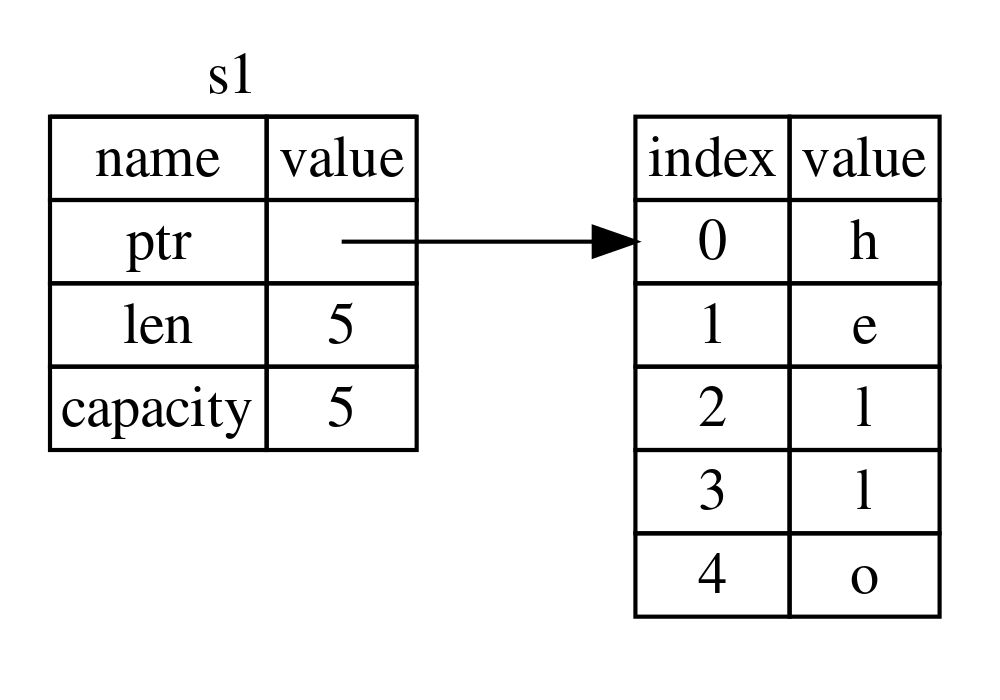
\includegraphics[width=0.5\textwidth]{figures/string-memory-rep.png}
    \caption{Representation of the memory layout of a string in Rust}
    \label{fig:string-memory-rep}
\end{figure}

When s1 gets copied into s2, only the pointer in the stack is copied, so that the memory layout of the program will look like the one in figure \ref{fig:string-memory-rep2}.

\begin{figure}[h]
    \centering
    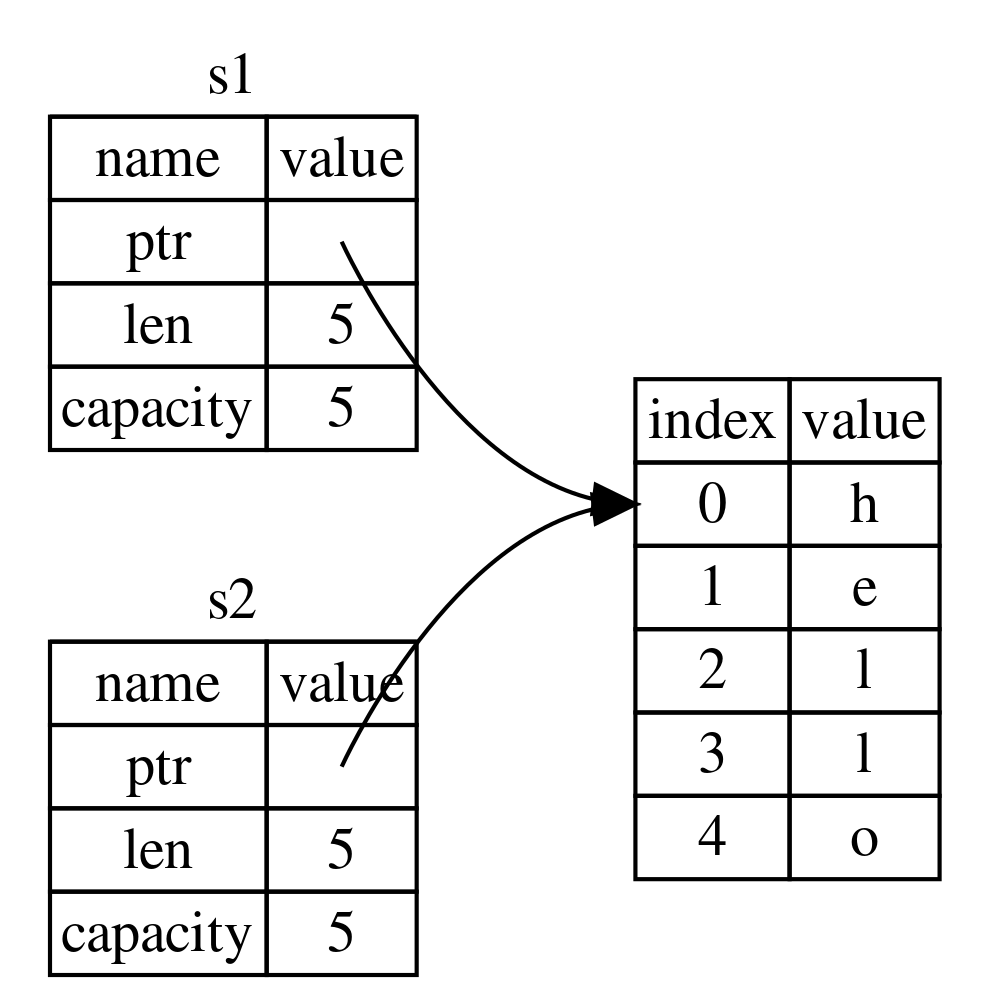
\includegraphics[width=0.5\textwidth]{figures/string-memory-rep-2.png}
    \caption{Representation of the memory layout of a string in Rust after the copy}
    \label{fig:string-memory-rep2}
\end{figure}

According to the ownership rules, when s1 and s2 go out of scope, one may think that the memory will be freed twice, causing a double-free error. However, in reality, after the copy, the compiler
will not consider s1 to be valid anymore, so when s1 goes out of scope, the memory will be freed only once, as shown in figure \ref{fig:string-memory-rep3}.

\begin{figure}[h]
    \centering
    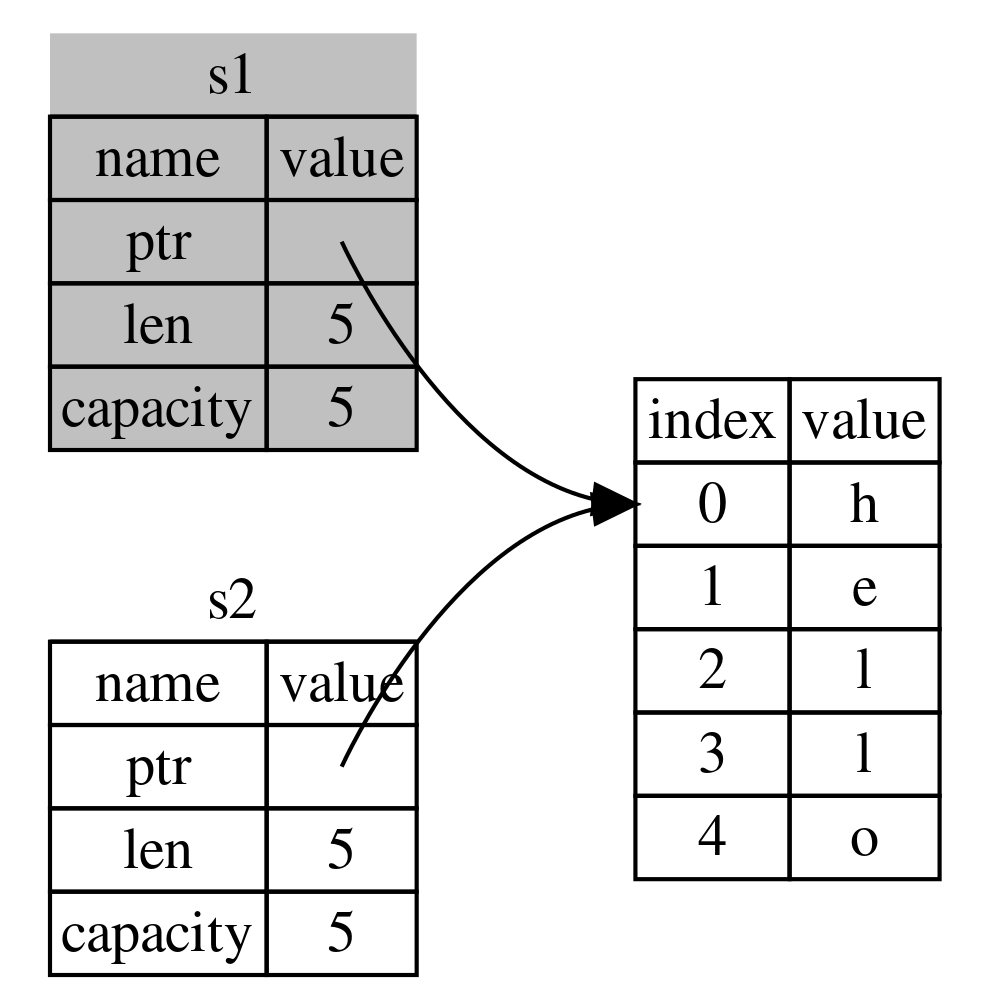
\includegraphics[width=0.5\textwidth]{figures/string-memory-rep-3.png}
    \caption{Representation of the memory layout of a string in Rust after the copy and the end of the scope of s1}
    \label{fig:string-memory-rep3}
\end{figure}

In this case, it is said that the variable s1 has been \textit{moved} into s2. This means that s1 is no longer valid and cannot be used anymore.
This happens because, by default, Rust doesn't create deep copies of variables of types that don't have a known size at compile time. After all, creating a deep copy of such
a variable would cause the allocation of a new memory block on the heap, an expensive operation both in terms of execution time and memory usage. If the developer
needs to create deep copies of variables stored in the heap, they can explicitly use the \textit{clone} method, which will create a new memory block on the heap and copy the data into it.

\subsubsection{Ownership and Functions}
Similarly to what happens during the variable assignment, passing a variable to a function will cause it, depending on its type, to be moved or copied, as shown in the listing \ref{lst:func_own_1}.

\lstinputlisting[language=Rust, label={lst:func_own_1}]{listings/function_ownership_ex1.rs}

Returning values from functions will also cause ownership to be transferred, as shown in the listing \ref{lst:func_own_2}.

\lstinputlisting[language=Rust, label={lst:func_own_2}]{listings/function_ownership_ex2.rs}

\subsubsection{References and Borrowing}
Instead of taking ownership of a variable and then returning it to the caller, it is possible to pass a reference to the variable to the function, so that the function can use the variable without taking ownership of it.
For a function to take a reference to a variable, it is sufficient to prefix the type definition of the variable with an ampersand (\&).
By default, references are immutable, meaning that the function cannot modify the value of the variable. If the function needs to modify the value of the variable, it is possible to take a mutable reference to it by using the \&mut keyword.

\subsection{Functional Features of Rust}
In this subsection, we will discuss some of the \ac{fp}-adjacent features of Rust.

\subsubsection{Product Types}
In FP, product types are types that combine n values of possibly different types. In Rust, it is possible to define Product types by using the \textit{struct} keyword. In particular, one can define a product type in two ways as shown in the listing \ref{lst:product_types}.

\lstinputlisting[language=Rust, label={lst:product_types}]{listings/product_types.rs}

It is also possible to add functionality to the ADTs created by using the \textit{impl} keyword, as shown in the listing \ref{lst:product_types_impl}.

\lstinputlisting[language=Rust, label={lst:product_types_impl}]{listings/product_types_impl.rs}

\subsubsection{Sum Types and Pattern Matching}
In FP, a sum type represents a choice between some types. In Rust, we can define Sum types by using the \textit{enum} keyword. It is also possible to perform pattern matching over a sum type, as it is shown in the listing \ref{lst:sum_types}.

\lstinputlisting[language=Rust, label={lst:sum_types}]{listings/sum_types.rs}

\subsubsection{Polymorphism}
Rust supports polymorphism through traits. Rust's traits are similar to Haskell's typeclasses and they allow us to define a particular functionality that a particular type has.
For example, we can implement Haskell's Show typeclass in Rust as shown in the listing \ref{lst:polymorphism}.

\lstinputlisting[language=Rust, label={lst:polymorphism}]{listings/polymorphism.rs}

\subsubsection{Lambdas and Closures}
In FP, lambda functions or anonymous functions, are functions that are not bound to a name. Moreover, closures are lambda functions that can "capture" the environment in which they are defined.
In Rust, both lambdas and closures are supported, though they are both called closures. Like in other languages, Rust closures can be assigned to variables and passed to functions.
When defining a closure in Rust, it is important to reason about the ownership of the variables that are captured by it. The listing \ref{lst:closures} shows some examples of closures in Rust.

\lstinputlisting[language=Rust, label={lst:closures}]{listings/closures.rs}

\subsubsection{Iterators}
The Iterator pattern allows to traverse collection of elements in a particular manner, performing some task on each element in turn. The iterator is responsible for the traversal logic
so that the developer doesn't need to reimplement it each time. In Rust, the Iterator pattern is implemented through the \textit{Iterator} trait, which is implemented by the standard library's collections:

\begin{lstlisting}[language=Rust]
    trait Iterator {
        type Item;
        fn next(&mut self) -> Option<Self::Item>;
        //Other default methods omitted
    }
\end{lstlisting}

The developer can also implement the Iterator trait for his custom types, enabling many functionalities that are divided into the following categories:

\begin{itemize}
    \item \textbf{Consumer Adaptors}: these are methods that take ownership of the iterator because they traverse it using its next method, thus consuming it. Examples of consumer adaptors are reducing methods like \textit{sum};
    \item \textbf{Iterator Adaptors}: these are methods that don't take ownership of the iterator, since they take an iterator and return another, modified one. An example of an iterator adaptor is the \textit{map} method, which applies a function to each element of the iterator;
\end{itemize}

\subsection{Why Rust}
As shown in the previous sections, Rust is a general-purpose programming language designed with a focus on safety, speed and efficiency. These design principles, coupled with high-level features
more adjacent to functional programming than to low-level programming, making Rust a good candidate for developing \ac{ac} implementations that can run on thin devices.


\section{Towards a Rust-based AC Implementation: the RustFields Project}
The RustFields Project\cite{001} was the first attempt to bring \ac{ac} to thin devices in the Rust programming language. The project aimed to reach its goals by developing two lines of research:
\begin{itemize}
    \item A pure, Rust-based implementation of AC in the same vein as the ScaFi framework;
    \item A mixed approach that aims to mix ScaFi's highly expressive API with Rust's performance and efficiency;
\end{itemize}

\subsection{RustFields Architecture}
As stated in the official documentation of the project: \\
``    Since the project was meant as an exploration of different options for bringing aggregate programming into native contexts, we decided to explore both solutions. The resulting architecture reflects this choice: in fact, we decided to develop a standalone aggregate programming framework in the Rust language, while also experimenting different ways to integrate it with the Scala ScaFi’s ecosystem.
''

The resulting architecture reflects this choice and this is made evident in the diagram in figure \ref{fig:rustfields-architecture}.

\begin{figure}[h]
    \centering
    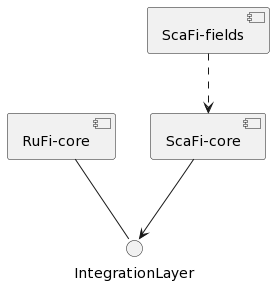
\includegraphics[width=0.5\textwidth]{figures/diagrams/img/rustfields-full-architecture.png}
    \caption{The RustFields Architecture}
    \label{fig:rustfields-architecture}
\end{figure}

In the architecture diagram shown in figure \ref{fig:rustfields-architecture}, the RuFi-core is responsible for implementing in Rust the core concepts of the new \ac{ac} implementation,
structured in a way that is somewhat similar to the ScaFi's core. Then, an \textit{integration layer} was built on top of the Rust core to allow communication
between Scala and Rust code. From then, the project development was divided into two main branches:
\begin{itemize}
    \item The expansion of the RuFi core, which aimed to serve as a base for a fully-fledged \ac{ac} implementation in Rust;
    \item The development of the integration layer, aimed to bring the best of both worlds by allowing the developer to use the expressive API of ScaFi with the performance and efficiency of Rust.
\end{itemize}

The design of the RuFi-core component is of particular interest since this thesis aims to expand it and further develop an \ac{ac} implementation in Rust.

\subsection{RuFi-core Design}
As stated in the previous sections regarding the architecture of RuFi-core, it was decided to stick as much as possible to the original architecture of ScaFi-core.
The RuFi-core architecture is shown in figure \ref{fig:rufi-core-architecture}.

\begin{figure}[h]
    \centering
    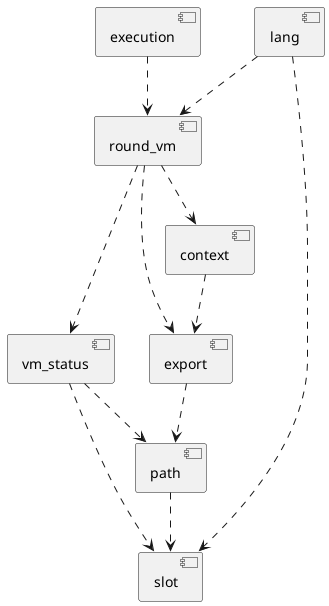
\includegraphics[width=0.5\textwidth]{figures/diagrams/img/rufi-core-architecture.png}
    \caption{The RustFields Architecture}
    \label{fig:rufi-core-architecture}
\end{figure}

\subsection{The Language}
RuFi-core's language implementation
%! Author = leona
%! Date = 09/02/24
% !TeX root = ../thesis-main.tex

\chapter{Analysis and Requirements}
\label{chap:requirements}
%! Author = leona
%! Date = 09/02/24
% !TeX root = ../thesis-main.tex

\chapter{Design}
\label{chap:design}

%! Author = leona
%! Date = 09/02/24
% !TeX root = ../thesis-main.tex

\chapter{Implementation}
\label{chap:Implementation}
This chapter aims to provide an overview of important implementation choices, as well as highlight the technologies used to develop the RuFi framework.

\section{Crate Structure}
At the highest level, the framework consists of multiple \textit{library crates}. In Rust, a crate is a standalone module that can be included as a dependency inside a project via
the \texttt{cargo} package manager. There are three types of crates in Rust:

\begin{itemize}
    \item \textit{Binary crates} are crates that can be compiled into an executable.
          An example of a binary crate can be a program that runs on a device and utilizes the RuFi framework.
    \item \textit{Library crates} are crates that can be used as a dependency in other projects.
    \item \textit{Proc Macro crates} are library crates that expose procedural macros.
\end{itemize}

The development of RuFi followed a convention that is common in the Rust community for large projects, and that is the use of a \textit{workspace}.
A workspace is a directory that contains multiple Rust crates, and it is defined by a \texttt{Cargo.toml} file that lists the crates that are part of the workspace.
Apart from this detail, each crate inside the workspace is a standalone Rust project with its specific dependency management and build configuration.
In particular, there are five different library crates in the RuFi workspace:

\begin{itemize}
    \item \texttt{rf-core} contains the RuFi core implementation.
    \item \texttt{rf-distributed} contains the RuFi distributed implementation.
    \item \texttt{rf-gradient} contains the implementation of the gradient aggregate program.
    \item \texttt{rf-distributed-impl} contains an implementation for the traits defined inside rf-distributed.
    \item \texttt{rufi} has a dependency on all the other crates and re-exports them under a common namespace. Thanks to Rust conditional compilation,
          it is possible to conditionally include or exclude entire modules from the dependency tree via the mechanism of \texttt{cargo features}, making this
          crate a convenient tool to access all the framework functionalities in a single, configurable dependency.
\end{itemize}

\section{RuFi Core}
This section will provide an overview of the implementation details for the RuFi core crate.

\subsection{RoundVM}
One of the most important functions of the RoundVM is the \textit{nest} function. 

\subsection{Language}

\section{RuFi Distributed}

\section{Networking}


\section{RuFi Gradient}
The RuFi Gradient crate contains an important example of what an aggregate program in RuFi can be and what it looks like. Since one of the core premises of \ac{fc} is to
provide key and reusable building blocks for aggregate computations, an aggregate program is nothing more than a function that combines these building blocks to achieve the
desired behavior. The aggregate program could then be used as a building block in a larger aggregate program, and so on.

The listing \ref{lst:rufi_gradient} shows the implementation of the RuFi Gradient aggregate program:

\lstinputlisting[language=Rust, label={lst:rufi_gradient}]{listings/rufi_gradient.rs}

The core functions used in this program are:

\begin{itemize}
    \item \textit{rep}: the operator that denotes a dynamically changing field;
    \item \textit{mux}: a branch variant that computes both the branches and returns the result of the branch that is selected by the condition. Since both branches of the operators
          are executed by the device, this construct does not restrict the domain like the \textit{branch} operator. Instead, it is used for simple conditional expressions;
    \item \textit{foldhood plus}: a variant of the foldhood operator that excludes the device from its neighborhood.
\end{itemize}

The \textit{is source} function calls the Virtual Machine and reads a sensor that establishes if the device is a source.
The aggregate program itself is a rep operation that has an initial value for the distance d equal to $0.0$.
Then, inside the repetition, there is a \textit{mux} call that returns a value of $0.0$ if the device is a source or else an aggregation between neighboring values is performed via the \textit{foldhood plus} builtin, resulting in the minimum distance $d + 1.0$ being kept as a result of the whole computation.
In this way, the immediate neighbors of the source will compute a value of $0.0 + 1.0$, and the neighbors of the neighbors will compute $1.0 + 1.0$, and so on.
For non-source devices that are not indirect neighbors of the source, the final result will be the starting value for the foldhood operator of $f64::INFINITY$.
%! Author = leona
%! Date = 09/02/24
% !TeX root = ../thesis-main.tex

\chapter{Validation}
\label{chap:validation}

The validation for this thesis' work has been done on multiple axes, which will be described in this chapter.

\section{Unit Testing}
The first layer of testing is the ``Unit Testing''. In computer science, this term refers to the act of analyzing and scrutinizing the smallest units of software possible.
This thesis adheres to Rust's unit testing practices: each public module that is part of the library has a corresponding and private testing module, annotated with the
conditional compilation macro ``\#[cfg(test)]'', denoting this is a module that is only compiled when the test suite is run.\\
Inside this module, it is possible to write test functions by annotating them with the ``\#[test]'' attribute. These functions can then be run with the ``cargo test'' command.\\
As such, each module in the RuFi library crates has a corresponding testing module containing unit test functions for them. For example, the listing \ref{lst:unit_test} shows the unit tests for the
vm\_status module.

\lstinputlisting[language=Rust, label={lst:unit_test}]{listings/unit_test.rs}

\section{Integration Testing}
Unit testing is a crucial practice in the development of software artifacts, but testing each component in isolation is not sufficient to analyze every aspect of the software produced.
Another important practice is the act of testing some or many components together, to ensure that their behavior when interacting is the one expected, which is called ``Integration Testing''.
Again, this thesis adheres to Rust's integration testing practices: each library crate has a corresponding ``tests'' directory, where integration tests are written. These tests are run with the ``cargo test'' command, just like their unit counterpart.\\
Inside the tests directory, it is possible to create various source files for testing. Each file is isolated from one another and is external to the library since it is compiled as an individual crate: this means that the
code inside these test files utilizes the library via its public API just like any other client code.\\
The listing \ref{lst:integration_test} shows an example of an integration test for the RuFi library that combines features coming from the RoundVM, Export and Language.

\lstinputlisting[language=Rust, label={lst:integration_test}]{listings/integration_test.rs}

\section{User Acceptance Testing}
A third axes along which the thesis' work has been validated is the ``User Acceptance Testing'', which refers to the practice of testing the software in a real-world scenario.
In particular, this involved the development of a demo project that exploits the RuFi framework to execute a gradient aggregate program within a network of 5 devices, each one
represented by a process running on a machine. At an application level, the topology is linear, meaning each device $i$ is a neighbor of the devices $i+1$ and $i-1$, excluding 1 and 5
which are the extremes of the topology. At a deployment level, there are four processes each one simulating a device running on a Desktop PC, while the fifth runs on a Raspberry Pi 3.\\
Each process communicates with the others through the MQTT protocol via the public Mosquitto MQTT broker. A graphical representation of the network is shown in figure \ref{fig:network_topology}.

\begin{figure}[ht!]
    \centering
    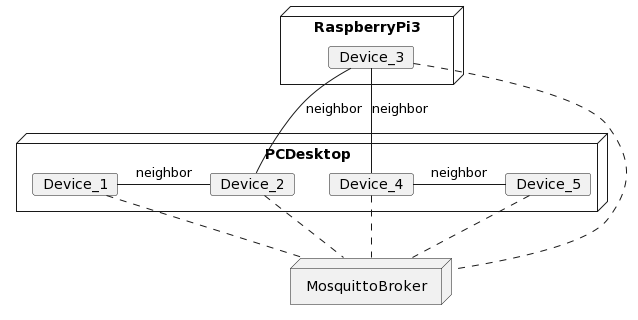
\includegraphics[width=0.8\textwidth]{figures/diagrams/img/deployment-demo.png}
    \caption{Network Topology}
    \label{fig:network_topology}
\end{figure}

\section{Memory Profiling}
Another important aspect to consider while implementing a framework that aims to bring \ac{ac} to thin devices is memory usage. Although a deep and comprehensive analysis of
the memory usage of the RuFi framework is beyond the scope of this thesis, a simple memory profiling with a particular focus on memory allocation spikes has been done to ensure that the framework does not consume an excessive amount of memory.
In particular, the profiling has been executed for three different execution cycles of the gradient aggregate program: 100, 300 and 500, at a frequency of 60mhz and for two devices:
the device number 1 and the device number 3. These devices have been chosen because they have a different amount of neighbors, which means we can see how processing multiple neighboring messages
can affect memory usage.

The results are shown in figure \ref{fig:memory_profiling}. The first group of columns shows the memory usage for the device number 3, while the second group shows the memory usage for the device number 1.

\begin{figure}[ht!]
    \centering
    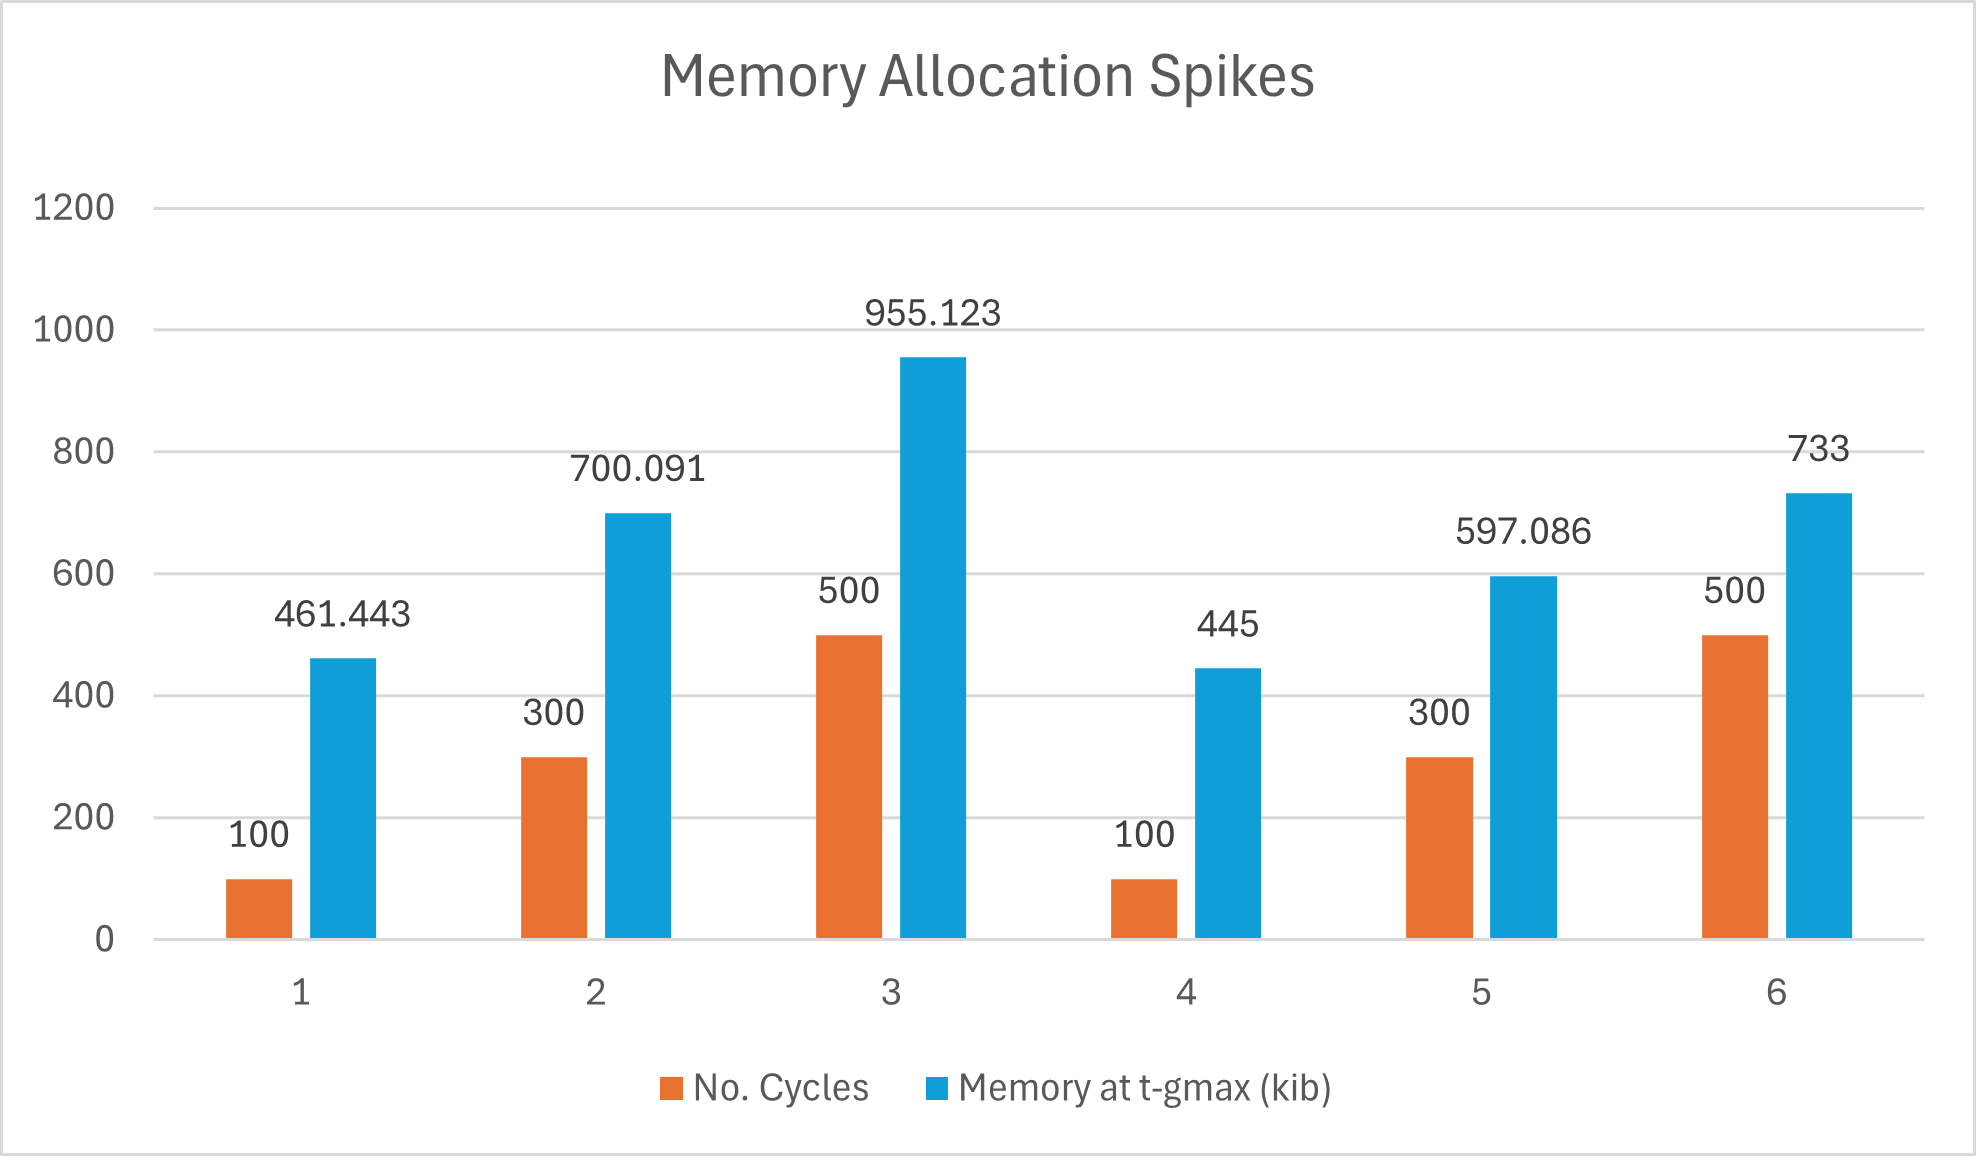
\includegraphics[width=0.8\textwidth]{figures/mem-spikes.png}
    \caption{Memory profiling for the devices 3 and 1.}
    \label{fig:memory_profiling}
\end{figure}

As we can see, the spike memory usage for the device with only one neighbor rises much more slowly than the one with two neighbors.
%! Author = leona
%! Date = 03/03/24
% !TeX root = ../thesis-main.tex

\chapter{Conclusion}
\label{chap:conclusions}
In this thesis, we have presented the design and development of a distributed execution platform for the RustFields framework, which has the ultimate goal of bringing Aggregate Computing to resource-constrained devices.
Starting by establishing a solid base regarding the context, paradigms and state-of-the-art for Aggregate Computing and a solid foundation of the Rust programming language concepts and idioms,
we were able to identify a set of requirements and goals for this thesis project, which were then used as a guide during the design and development phases.
Our analysis of the current state of the RustFields project has highlighted the need for validation and improvement of the current core library, as well as the need for a new module that would enable
the distributed execution of Rust-based aggregate programs. With these considerations in mind, we started by thoroughly testing the core of the framework via unit testing and integration testing, as well as developing
a set of macros that will help reduce the amount of boilerplate code one needs to write when defining an aggregate program. Then, we proposed the design of the new RustFields framework, RuFi, highlighting first the architectural design of the project and its main
components, and then delving into the detailed design of such components. These designs were then used as a guideline for the implementation phase, where we highlighted some important tactical choices that were made.
We also started collecting experimental data on memory usage of the current RustFields framework, which will be useful for future research and improvements.

\section{Current Limitations}
As of now, although the main goal of the thesis of providing a distributed execution platform for the RustFields framework has been achieved, the higher-level objective of bringing \ac{ac} on all thin devices is still not fully accomplished.
Experiments on running the current RuFi framework in very resource-constrained devices like the Esp32 have shown that the current implementation is not yet suitable for such devices, as the memory usage is still too high, highlighting the need
for further research and improvement on the memory footprint of such a framework.

\section{Future Work}
The previous analysis of the limitations of the current RuFi implementation has already suggested an important objective for future work.
Nevertheless, there are also other interesting directions to consider, such as:

\begin{itemize}
      \item implementation of a proprietary Mqtt broker: currently, RuFi relies on a public Mqtt broker for the communication between devices.
            However, having a proprietary Mqtt broker would allow for more control over the communication and the possibility of implementing more advanced features;
      \item improve further the RuFi API and DSL: the current improvements on the developer experience of the RuFi API and DSL are solely based on simple Rust declarative macros and although they eliminate
            some of the boilerplate code, they are still not as user-friendly as higher-level DSLs like \ac{scafi}. A possible future line of research could be leveraging the more powerful Rust procedural macros, a subject that was not expanded in this thesis
            but could offer many opportunities to improve the RuFi DSL.
\end{itemize}
%----------------------------------------------------------------------------------------
% BIBLIOGRAPHY
%----------------------------------------------------------------------------------------

\backmatter

\nocite{*} % comment this to only show the referenced entries from the .bib file

\bibliographystyle{alpha}
\bibliography{bibliography}

\end{document}